\begin{frame}{\acrshort{fpga} introduction}
    \begin{itemize}
        \item Field Programmable Gate Arrays
        \item Configurable Logic Block Matrix
        \item Variable granurality
        
    \end{itemize}
\end{frame}


\begin{frame}{\acrshort{fpga} introduction}
    \begin{itemize}
        \item \acrfull{fpga}
        \item Xilinx Spartan 7 \cite{sp701} \cite{fpga_resources}
            \begin{itemize}
                \item x \gls{lut}
                \item \aqnote{posar resources (?) justificacio de decisions de disseny mes endavant}
            \end{itemize}
    \end{itemize}
\end{frame}

\begin{frame}{Xilinx Spartan 7 \cite{sp701} \cite{fpga_resources}}
    \column{0.5\textwidth} % Left column and width
	    \begin{itemize}
	    \item Chip xc7s100 serie %https://www.mouser.es/ProductDetail/?qs=unwgFEO1A6sZ6LzV7v6FSA%3D%3D
	    \begin{itemize}
	    	\item 102400 LE %Logic elements: smallest units of logic. LEs  provide advanced features with efficient logic like LUT
	   	 \item 16000 ALM %adaptive logic module: more complex boolean functions with/without registers
	    	\item 400 I/O  per second %Input output operations per second 
	    \end{itemize}
	\end{itemize}
\column{.5\textwidth} % Right column and width

\begin{figure}[!ht]
    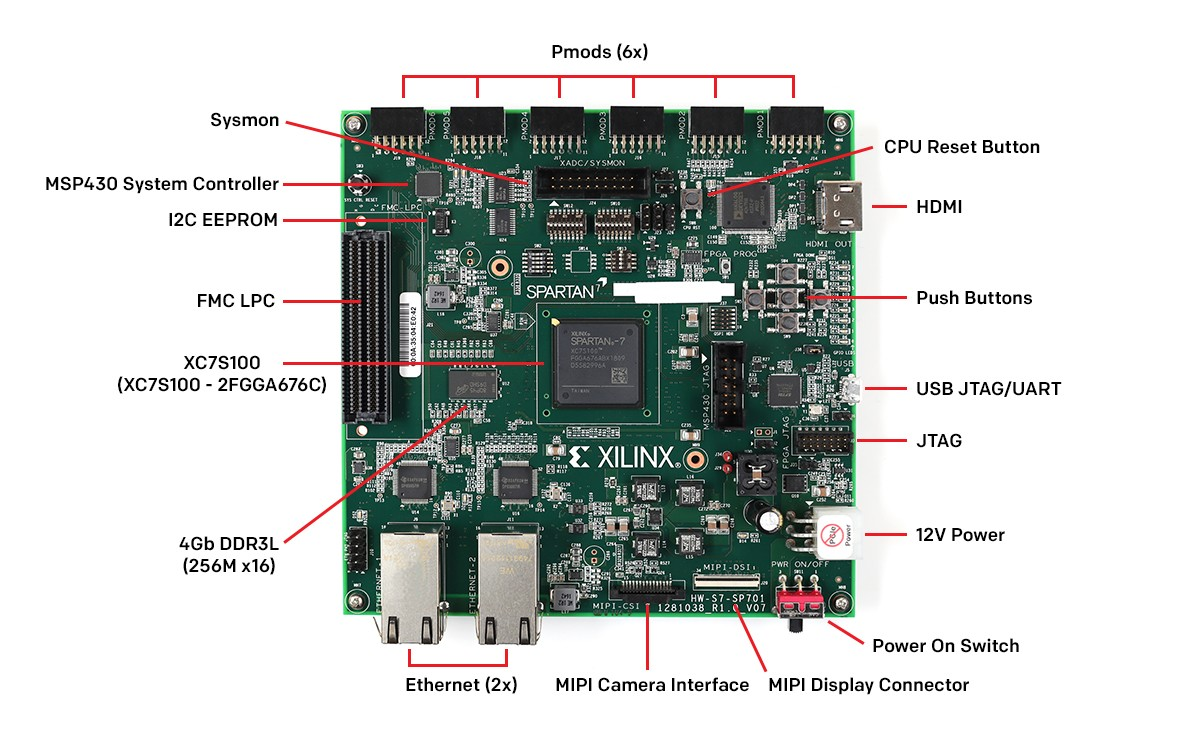
\includegraphics[width=1\linewidth]{images/spartan7.jpg}
\end{figure}
\end{columns}
\end{frame}
